\documentclass[12pt,compress,ngerman,utf8,t]{beamer}
\usepackage[ngerman]{babel}
\usepackage{calc}
\usepackage{ragged2e,wasysym,multicol,mathtools,txfonts,tikz,ifthen}
\usepackage[protrusion=true,expansion=true]{microtype}
\usepackage{booktabs}
\usepackage{multimedia}
\hypersetup{colorlinks=true}

\graphicspath{{images/}}

\title[Nullwissenbeweise]{Die wundersame Welt der \\ Nullwissenbeweise}
\author[Ingo Blechschmidt, Anna Rubeck]{\scriptsize
\vspace*{-1em} \\
\textcolor{white}{\textbf{UniMentoSchule am 2. März 2018} \\
\textbf{Fragen sind jederzeit willkommen! Bitte nicht bis zum Ende
aufsparen.} \\
\medskip
Ingo Blechschmidt und Anna Rubeck \\
Lehrstuhl für Algebra und Zahlentheorie \\
Institut für Mathematik \\
Universität Augsburg}}

\useinnertheme[shadow=true]{rounded}
\useoutertheme{split}
\usecolortheme{orchid}
\usecolortheme{whale}
\setbeamerfont{block title}{size={}}

\useinnertheme{rectangles}

\usecolortheme{seahorse}
\definecolor{mypurple}{RGB}{150,0,255}
\setbeamercolor{structure}{fg=mypurple}
\definecolor{myred}{RGB}{150,0,0}
\setbeamercolor*{title}{bg=myred,fg=white}
\setbeamercolor*{titlelike}{bg=myred,fg=white}

\newcommand{\redheart}{\scalebox{1.2}{\textcolor{mypurple}{$\varheartsuit$}}}

\usefonttheme{serif}
\usepackage[T1]{fontenc}
\usepackage{libertine}

\setbeamertemplate{navigation symbols}{}

\setbeamertemplate{title page}[default][colsep=-1bp,rounded=false,shadow=false]
\setbeamertemplate{frametitle}[default][colsep=-2bp,rounded=false,shadow=false,center]

\newcommand{\hil}[1]{{\usebeamercolor[fg]{item}{\textbf{#1}}}}
\setbeamertemplate{frametitle}{%
  \vskip1em%
  \leavevmode%
  \begin{beamercolorbox}[dp=1ex,center]{}%
      \usebeamercolor[fg]{item}{\textbf{\textsf{\Large \insertframetitle}}}
  \end{beamercolorbox}%
}

\setbeamertemplate{footline}{%
  \leavevmode%
  \hfill%
  \begin{beamercolorbox}[ht=2.25ex,dp=1ex,right,rightskip=1mm,leftskip=1mm]{}%
    \usebeamerfont{date in head/foot}
    Die wundersame Welt der Nullwissenbeweise \hfill
    \insertframenumber\,/\,\inserttotalframenumber
  \end{beamercolorbox}%
  \vskip0pt%
}

\newcommand{\withsource}[2]{\begin{center}#1\\\tiny #2\end{center}}

\setbeameroption{hide notes}
\setbeamertemplate{note page}[plain]

% Taken from Todd Lehman (CC-BY-SA) at https://tex.stackexchange.com/a/44920/32372

\newcommand{\setisprime}[1]{
  % Sets \isprime based on #1.
  \ifnum#1=1 \gdef\isprime{0} \else \gdef\isprime{1} \fi
  \foreach \sip in {2, 3,5,...,#1} {
    \pgfmathparse{\sip*\sip>#1? 1:0}
    \ifthenelse{\pgfmathresult=1}{
      % Early-out if \sip^2 > #1.
      \breakforeach
    }{
      % Otherwise test if \sip divides #1.
      \pgfmathparse{Mod(#1,\sip)==0? 1:0}
      \ifthenelse{\pgfmathresult=1}{
        \gdef\isprime{0}
        \breakforeach
      }{}
    }
  }
}

\newcommand{\setxy}[1]{
  % Sets \x and \y to loction of cell #1.
  \pgfmathtruncatemacro{\x}{Mod(#1-1,\cols)}
  \pgfmathtruncatemacro{\y}{(#1-1) / \cols}
  \pgfmathtruncatemacro{\y}{\cols - 1 - \y}
  \pgfmathparse{2.5*(\x+.5)}\let\x\pgfmathresult
  \pgfmathparse{2.5*(\y+.5)}\let\y\pgfmathresult
}

\newcommand{\numlabel}[2]{
  % Draws label #2 at cell #1.
  \setxy{\n}
  \node[fill=none, text=black] at (\x,\y) {#2};
}

\newcommand{\drawpolygon}[2]{
  % Draws polygon with #2 vertexes at cell #1.
  \setxy{#1}
  \ifthenelse{#2>1}{ % Polygon must have at least 2 sides.
    \ifthenelse{#2<30}{ % Draw polygon if it has a small number of sides.
      \filldraw (\x,\y) +(90:1)
      \foreach \drawi in {1,...,#2} {-- +(\drawi/#2*360+90:1)} -- cycle;
    }{ % Else approximate with circle.
      \filldraw (\x,\y) circle(1);
    }
  }{}
}

\newcommand{\setpolygoncolor}[1]{
  % Sets color based on #1.
  \gdef\polycolor{black}
  \ifnum#1=2\gdef\polycolor{black!50!white}\fi
  \ifnum#1=3\gdef\polycolor{yellow!95!red}\fi
  \ifnum#1=5\gdef\polycolor{yellow!0!red}\fi
  \ifnum#1=7\gdef\polycolor{blue!75!green}\fi
  \ifnum#1=11\gdef\polycolor{blue!70!red}\fi
  \ifnum#1=13\gdef\polycolor{blue!40!red}\fi
  \ifnum#1=17\gdef\polycolor{green!50!blue}\fi
  \ifnum#1=19\gdef\polycolor{green!80!black}\fi
  \ifnum#1=23\gdef\polycolor{green!50!red}\fi
  \ifnum#1=29\gdef\polycolor{yellow!50!black}\fi
  \ifnum#1=31\gdef\polycolor{orange!50!black}\fi
  \ifnum#1=37\gdef\polycolor{red!50!black}\fi
  \ifnum#1=41\gdef\polycolor{purple!50!black}\fi
  \ifnum#1=43\gdef\polycolor{blue!50!black}\fi
  \ifnum#1=47\gdef\polycolor{green!50!black}\fi
  \ifnum#1=53\gdef\polycolor{white!50!black}\fi
  \ifnum#1=59\gdef\polycolor{white!50!black}\fi
  \ifnum#1=61\gdef\polycolor{white!50!black}\fi
  \ifnum#1=67\gdef\polycolor{white!50!black}\fi
}

\newcommand{\sieve}[2]{
  \def\cols{#1}
  \def\rows{#2}
  \begin{tikzpicture}[scale=.5,anchor=center]
  \pgfmathtruncatemacro{\nmax}{\rows * \cols}

  \foreach \n in {1,...,\nmax} {
    \begin{scope}[fill=gray, fill opacity=.05,
                  draw=gray, draw opacity=.10,
                  line width=4]
      \drawpolygon{\n}{\n}
    \end{scope}
    \setisprime{\n}
    \ifthenelse{\isprime=1}{
      \numlabel{\n}{\bf\n}
    }{
      \def\startintensity{.33}
      \def\incrintensity{.10}
      \def\intensity{\startintensity}

      \def\m{\n}
      \pgfmathtruncatemacro{\i}{\m / 2}

      % Divide \m by \i until \m is extinguished.
      % Increment \i each time it does not divide into \m.
      \whiledo{\m>1}{
        \setisprime{\i}
        \pgfmathparse{Mod(\m,\i)==0? 1:0}
        \ifthenelse{\pgfmathresult=1\and\isprime=1}{
          \setpolygoncolor{\i}
          \begin{scope}[fill=\polycolor, fill opacity=\intensity,
                        draw=\polycolor!85!black, draw opacity=\intensity,
                        line width=\intensity*1.5]
            \drawpolygon{\n}{\i}
          \end{scope}
          \pgfmathtruncatemacro{\m}{\m / \i}
          \pgfmathparse{\intensity + \incrintensity}\let\intensity\pgfmathresult
        }{
          \pgfmathtruncatemacro{\i}{\i - 1}
          \def\intensity{\startintensity}
        }
      }
      \begin{scope}[text=black, text opacity=.5]
        \numlabel{\n}{\scriptsize\n}
      \end{scope}
    }
  }

  \end{tikzpicture}
}


\begin{document}

{\setbeamertemplate{footline}{}
\usebackgroundtemplate{\begin{minipage}{\paperwidth}\vspace*{3.35cm}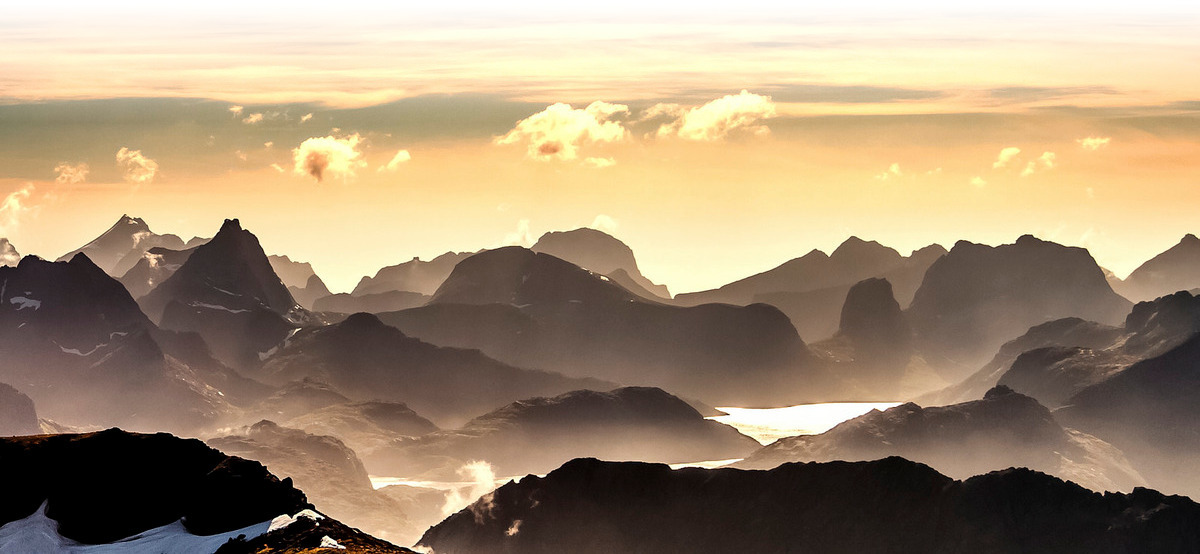
\includegraphics[width=\paperwidth]{freedom}
\\ \centering \tiny Foto: \href{https://www.flickr.com/photos/steinliland/14435047450/}{Stein Liland} (CC-BY-NC) \end{minipage}}
\begin{frame}
  \centering
  {\qquad\quad\!}
\includegraphics[width=0.25\textwidth]{gregor}
  \vspace*{-0.5em}

  \titlepage
\end{frame}}

\addtocounter{framenumber}{-2}


\section{Ein Rechentrick}

\begin{frame}{Ein Rechentrick}
  \vspace*{-1em}
  \begin{columns}[c]
    \begin{column}{0.2\textwidth}
      \withsource{
        
\includegraphics[width=\textwidth]{question-mark}
      }{
        Illustration: \\
        \href{https://commons.wikimedia.org/wiki/File:Question_mark_1.svg}{Nevit
        Dilmen/Wikipedia} (CC-BY-SA)
      }
    \end{column}

    \begin{column}{0.7\textwidth}
      \large\centering
      Was ist{\quad}
      \[ 1 + 2 + 3 + \cdots + 98 + 99 + 100? \]
    \end{column}
  \end{columns}

  \pause

  \begin{columns}[c]
    \begin{column}{0.2\textwidth}
      \withsource{
        
\includegraphics[width=\textwidth]{idea}
      }{
        Illustration: \\
        \href{https://commons.wikimedia.org/wiki/File:Crystal_Clear_app_ktip.svg}{Jacob
        Hnri 6/Wikipedia} (CC-BY-SA)
      }
    \end{column}

    \begin{column}{0.7\textwidth}
      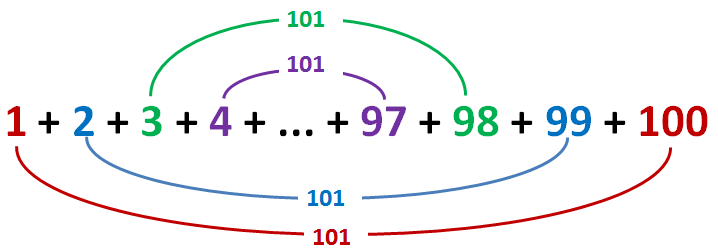
\includegraphics[width=\textwidth]{kleiner-gauss}
    \end{column}
  \end{columns}
\end{frame}

\begin{frame}{Primzahlen mögen die Sechs}
  \centering
  \vspace*{-0.5em}
  \withsource{\scalebox{0.7}{\sieve{6}{8}}}{Illustration:
  \href{https://tex.stackexchange.com/a/44920/32372}{Todd Lehman} (CC-BY-SA)}
\end{frame}


\section{Wo ist Walter?}

\begin{frame}{Wo ist Walter?}
  \centering
  
\includegraphics[height=0.8\textheight]{waldo}
\end{frame}


\section{Ali Baba}

\begin{frame}{Ali Baba}
  \centering
  \withsource{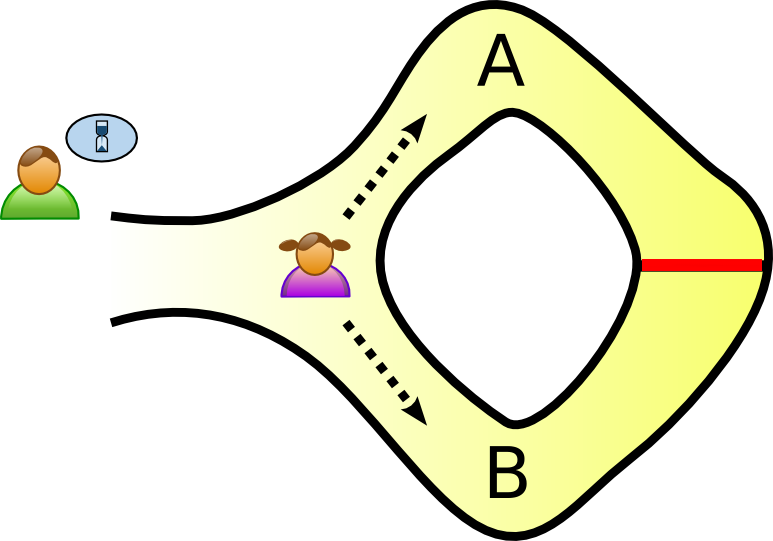
\includegraphics[height=0.7\textheight]{alibaba1}}{Illustration:
  \href{https://commons.wikimedia.org/wiki/File:Zkip_alibaba1.png}{Dake/Wikipedia} (CC-BY)}
\end{frame}


\appendix

\begin{frame}{Mathecamp}
  \centering
  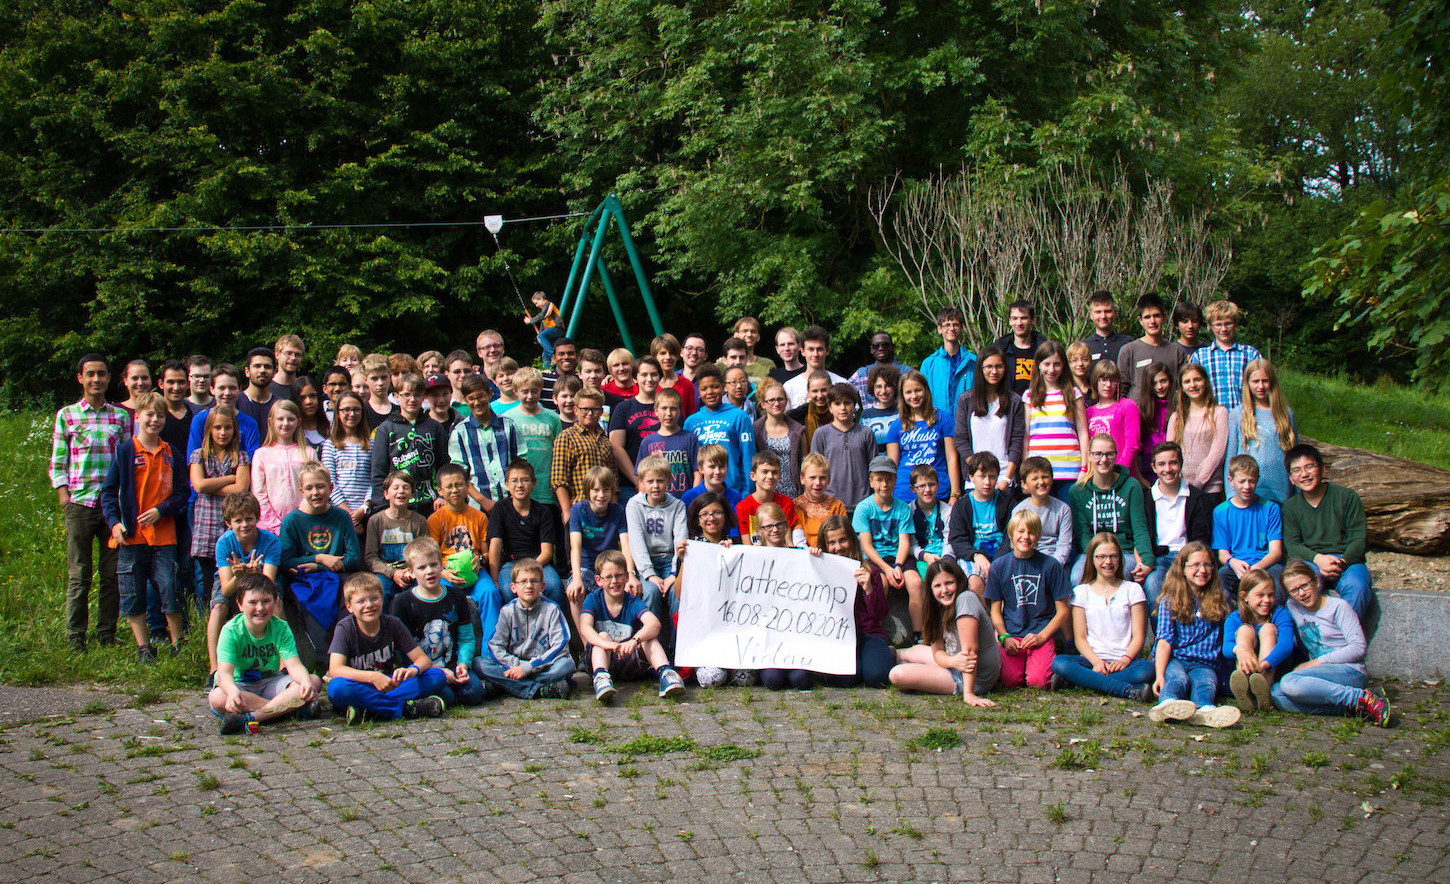
\includegraphics[width=0.9\textwidth]{mathecamp-gruppenfoto}
  \medskip

  \redheart{} 18. bis 26. August in Violau \redheart{}
\end{frame}

{\usebackgroundtemplate{\begin{minipage}{\paperwidth}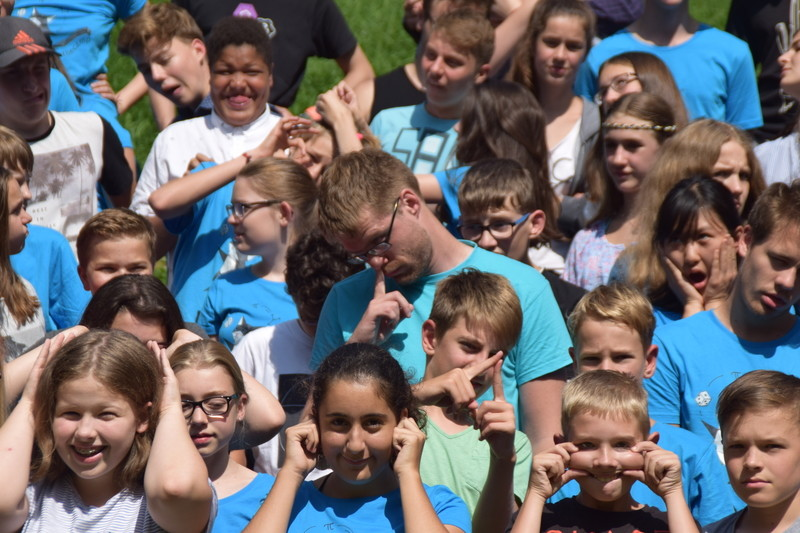
\includegraphics[height=\paperheight]{mathecamp-crazy}\end{minipage}}
\begin{frame}[plain]
\end{frame}

\addtocounter{framenumber}{-1}

\end{document}
